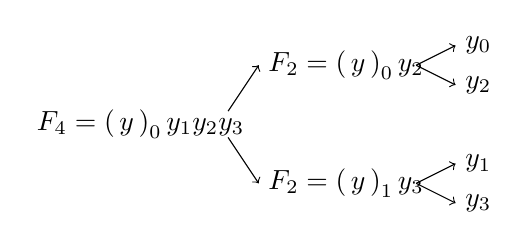
\begin{tikzpicture}[scale=0.5]
\node at (0,0) {$F_4 = \begin{pmatrix} y_0 \\ y_1 \\ y_2 \\ y_3  \end{pmatrix}$};

\draw[->, shorten <= 0.2cm] (2,0) -- (3, 1.5);
\draw[->, shorten <= 0.2cm] (2,0) -- (3,-1.5);

\node[right] at (3,1.5) {$F_2 = \begin{pmatrix} y_0 \\ y_2 \end{pmatrix}$};

\draw[->] (7,1.5) -- (8,2) node[right] {$ y_0 $};
\draw[->] (7,1.5) -- (8,1) node[right] {$ y_2 $};


\node[right] at (3,-1.5) {$F_2 = \begin{pmatrix} y_1 \\ y_3 \end{pmatrix}$};

\draw[->] (7, -1.5) -- (8, -1) node[right] {$ y_1 $};
\draw[->] (7, -1.5) -- (8, -2) node[right] {$ y_3 $};


\end{tikzpicture}